% Chapter Template

\chapter{Background} % Main chapter title

\label{Chapter2} % Change 2 to a consecutive number; for referencing this chapter elsewhere, use \ref{Chapter2}

Web applications have made a rapid progress over the last years in the field of both technologies used and architectural approach. A web application is consisted of a client and a web server. Client is considered to be, for example, a web browser in a mobile phone or in a desktop computer. Client sends a request to the server, where processes are performed depending on the request, and a response is sent back to the client. (\cite{Reference6}) As picture bellow reveals, client is making a request and server attempts to fulfill it by referring to a data base, performing calculations, controlling or sending another request to other servers. \par

\begin{figure}[h!]
	\begin{center}
		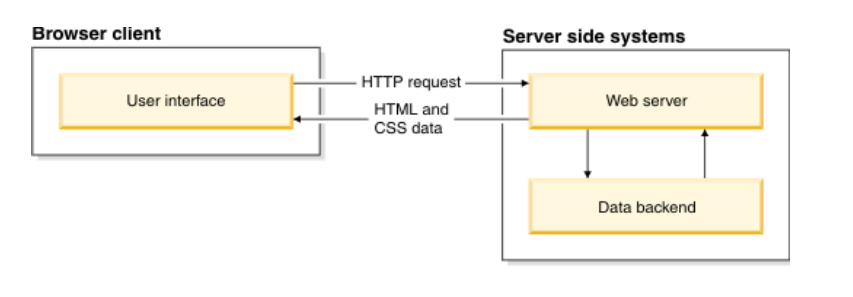
\includegraphics[scale=0.8]{images/web_structure.png}
	\end{center}
	\caption{Web application data transfer model}
\end{figure}

Functionalities can be spotted in the client side as well. Client can customize HTML DOM, Document Object Model structure used for accessing different elements, display interactive visualizations or alerts through the utilization of Javascript programming language. (\cite{Reference6}) \par

Architecture, which is a set of defined terms and rules used as instructions to build a web service, influence both software design and engineering. The choice of a web application's architectural design impacts on development time and maintenance costs, every-day's transactional performance, response times, continual application's flexibility and scalability. The architecture is selected based on the app's complexity, integration level, number of users and their geographical distribution, network's nature and long-term transactional needs. (\cite{Reference1})\par

\newpage
\subsection{Architectural Designs}
In the late 1950s, mainframe architecture was introduced. This architecture was designed for mainframe computers that are used to large-scale computing applications, such as data storage or customer statistics. Every kind of program and data was stored in a single machine and users could only reach this centralized computer only through the terminals' usage.

\begin{figure}[h!]
	\begin{center}
		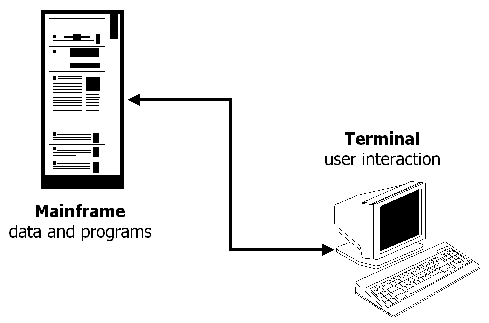
\includegraphics[scale=0.45]{images/mainframe.jpg}
	\end{center}
	\caption{Mainframe Architecture}
\end{figure}

In the 1980s, two-tier architecture was introduced due to the entry of network connected computers. In more details, this architectural approach consists of an application running in the client and interacting with the server as a database management system. In that perspective, client contains the presentation logic, navigation of the application, business rules and the database access. By changing the business rules in two-tier architecture, the client had to be modified and tested all over again, even in case the user interface is the same. For minimizing the costs of conversions, presentation logic and business rules had to be separated, fact that gained the principle of three-layer architecture.

\begin{figure}[h!]
	\begin{center}
		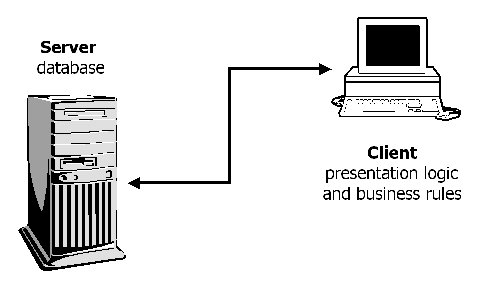
\includegraphics[scale=0.45]{images/two-tier_architecture.jpg}
	\end{center}
	\caption{Two-Tier Architecture}
\end{figure}

In a three-tier architecture, also referred as multi-tier, there are up to three interacting layers. System functionality is thereby distributed with each own of these tiers having a subset of responsibilities.

\begin{figure}[h!]
	\begin{center}
		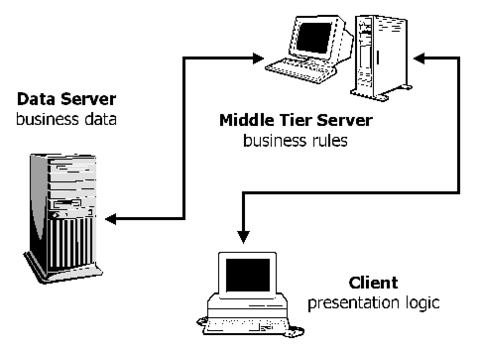
\includegraphics[scale=0.45]{images/three-tier_architecture.jpg}
	\end{center}
	\caption{Three-Tier Architecture}
\end{figure}

As the Figure 2.4 shows, first tier refers to the presentation logic, known as client, and includes user interface and input validation. Second tier or, in other words, middle tier or application server, provides data access and the business logic. Finally, third tier is the data server and provides business data and resources. The pros of three-layer architectural design is the ease replace or modification of any layer without influencing or changing the others. Another advantage is the load balancing that this separation of layers and the database functionality provides. (\cite{Reference3})

%----------------------------------------------------------------------------------------
%	SECTION 1
%----------------------------------------------------------------------------------------

\section{Three-layer Architecture}

Three-layer Architecture is a software architectural pattern in which the application is separated into three logical layers known as presentation, business logic and data storage layer. This architecture is adopted by client-server applications that have frontend, backend and database.(\cite{Reference2}) Data access and calculations required by the presentation layer, are part of the business logic layer and, for this purpose, calls to middle-tier servers are made. Middle-layer servers can be approached by various clients, which are from different applications as well. Each one of these tiers has specific responsibilities and can be handled independently. (\cite{Reference5}) \par

\begin{figure}[h!]
	\begin{center}
		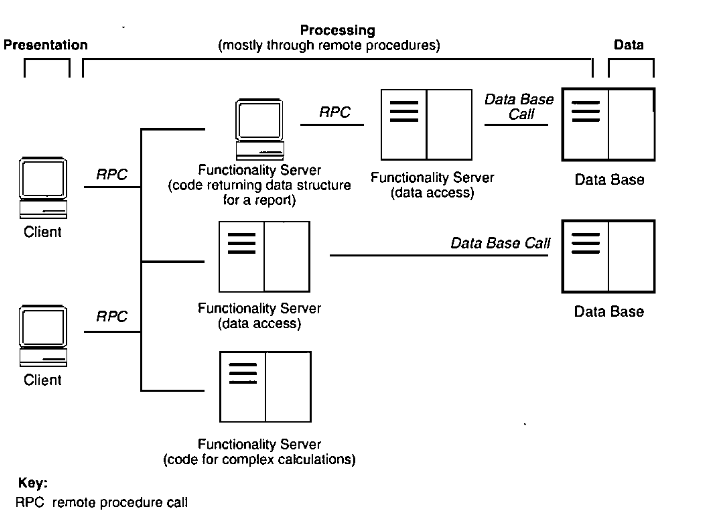
\includegraphics[scale=0.85]{images/three-layer-architecture-details.png}
	\end{center}
	\caption{Three-Tier Architecture}
\end{figure}

Interaction between client and server is succeeded mostly through the Remote Procedure Call, which is a way to describe calling mechanism among procedures and to exchange data via messages. In RPC, clients request data by passing parameters needed and specify data structure to received values in order the request to be fulfilled. \\
HTTP is the protocol used for messages' passing. HTTP stands for Hypertext Transfer Protocol through which resources are exposed across distributed systems. An HTTP request includes a body with the representation of resources required by the client. An architectural style that is based on RPC implementation is called Representational State Transfer. REST is implemented in client/server models where the client is gaining data or interacting with resources managed by server. \par

There are a lot of advantages adapting three-architecture layering design. First and foremost, modularity, having separate software entities allows each layer to be managed independently of the others.(\cite{Reference2}) This has as a result different groups of people to focus on different tiers, so as parallel development to be succeeded and people to become specialists. It has to be mentioned that skills needed for application development varies, and having some experts responsible for each tier can improve the general quality of the application.(\cite{Reference5})\par

Scalability of three-tier architectural pattern is another benefit. This architecture provides flexibility in resource distribution. In more details, servers are portable, and dynamically distributed and changed based on the application's requirements. (\cite{Reference5})  Each of the tiers scales horizontally in order trafficking and request demand to be supported. For example, scalability can be done by adding more Elastic Compute Cloud instances, which is a cloud service providing security and compute capacity, and load balancing to each layer. (\cite{Reference2}) \par

Another core profit of this distribution is that code units can be reusable. This logic minimize the maintenance costs, development efforts and the ability to easily switch technologies used. Moreover, there are various additional features that support modularized applications, which means that integrated security, server control and dynamic fault-tolerance are supported. (\cite{Reference5})\par

Security is easier to be performed in three-layer architecture. All of the interactions within the application are made through private Internet protocol addresses. Users access client/server systems via the presentation tier. The other two layers, server and database, are not exposed to network which offers protection, security and barriers against malicious users. Fault tolerant is also provided for adaption in any unexpected change. (\cite{Reference2})\par

In conclusion, this layering model is the most frequent architectural design and is defined as components' separation into different tiers. Each layer's components are abstract with limited dependences between them, reusable and easy maintained. (\cite{Reference2}) \par

\subsubsection{Presentation Layer}
Presentation layer or client is the user interface part of the application. In other words, this layer controls the interaction between user and system, and is also responsible for input validation. Presentation tier's infrastructure is exclusively related to interface elements. (\cite{Reference2})\par

\subsubsection{Business Logic Layer}
Business logic layer or server is the body of an application. This is related to how the service works and it is responsible for computations and connection between client and database. (\cite{Reference2}) Several server requests and data access is made through the middle tier instead of client, thus traffic, memory and disk storage requirements are minimized. (\cite{Reference5})\par

\subsubsection{Data Layer}
Data access layer or database is responsible for providing business data and resources. Data are stored in this layer and are accessed from other layers when it is needed. (\cite{Reference2})\par


\section{Rest}
Representative State Transfer is an architectural style for building networked hypermedia applications that are easy to implement, lightweight, maintainable and scalable. A service based on Rest architectural approach is called Restful. The main purpose of a Restful service is providing data access to the client through a window. By the term of data or resources, we mean everything that can be captured in a computer-based informational system, such as pictures, videos, Web pages or any other business information. (\cite{Reference7}) \par

Rest architectural style is based on four main principles. The first one is that resources are identified by URIs, which is a universal addressing space for resources and service exploration. Furthermore, the principle of uniform interface is the way resources are by using a set of four operations. More specifically, resources can be controlled by PUT, POST, GET, DELETE, which are for update, add, retrieve and remove actions. The next principle stands for self-descriptive messages. In other words, resources can be represented in a variety of formats depending on the requirements, such as JSON, XML, HTML or even plain text, and meta-data are also available in order caching to be controlled, transmitting errors to be detected and authentication to be performed. Last but not least, every interaction with a resource is stateless. This means that each request message is self-contained and there is no need of state transfer. (\cite{Reference8}) \par

HTTP is the protocol that is used in almost every Restful Web service and it is implementing the service with features of a uniform interface and caching. This protocol is giving the ability of communication between client and server through messages. Client sends a request to the server, and server returns a response to that request. (\cite{Reference7}) Rest APIs are the bridge between this communication, so as the client to get the resources needed from the server without knowing how the structure of Restful API works and vice versa. (\cite{Reference9}) \par

\begin{figure}[h!]
	\begin{center}
		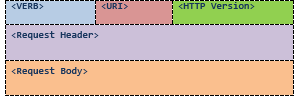
\includegraphics[scale=0.85]{images/httpFormat.png}
	\end{center}
	\caption{HTTP request format}
\end{figure}

In conclusion, Rest architectural approach is a lightweight infrastructure, where services can be built with minimum tooling and effort that leads to inexpensive and low barrier adoption. Restful Web services serve a large number of clients because of the caching and load balancing build of Rest, and have the ability to access resources without registration, and the advantage to optimize data in different formats. (\cite{Reference8}) \par

\section{Dynamic Pages}

Web application systems are using Web browsers for representing client. Web browsers interprets HTML, CSS and Javascript code, and communicate with server side through the usage of urls and HTTP protocol. In first place, static web pages were send to browsers and server's responsibility was to locate and send files, based on client's requests. Afterwards, dynamic pages were generated by servers via running software, and by clients via executable code. Thus, a lot different software development, such as languages, APIS, libraries or frameworks, were build to support dynamic pages' approach. Ajax, Javascript, Python, and much more other such development tools, are a good example. (\cite{Reference4}) \par

Ajax stands for "Asynchronous JavaScript And XML" and provides asynchronous requests for data transfer. By using Ajax, an application can dynamically update its page's content without the need of reloading the entire DOM all over again. In general, Ajax is a way to get a certain functionality by using web technologies on the client side, in order to create asynchronous applications. Ajax is different than JS frameworks or libraries which include a lot capabilities and functionalities along with Ajax. (\cite{Reference17}) \par

JavaScript is the language created to fulfill the need of client-based dynamic pages. JavaScript is being developed really quick and new versions of the language are often released, like the so called ECMAScript 2015, or namely ES6, and other more recent ones, like ES7. Generally, ECMAScript or ES is a standard formation body of JS scripting language with ES5, named also as ECMAScript 2014, to be the version all browsers understand. (\cite{Reference10}) As regards coding with JavaScript, developers prefer to use ES6 and its upgrades for coding. This is because these new versions mark a new generation of the referring language with a dozen of additional features compared to ES5, the previous version. For using new features implemented in ES6, there are programs like Babel that convert the newer syntax to ES5, that is browser-compatible. (\cite{Reference13}) \par

Moreover, new technologies based on JavaScript are regularly released. So, libraries and frameworks are inclined to make easier JS development and improve its capabilities. JavaScript's libraries exist for a long period of time and in 2006, they got popular for first time with jQuary. AngularJS and Ember, which are other JS frameworks, became known between 2010 and 2011. AngularJS was the first framework that composed routing and data binding in one. Ember followed and provided some improvements on AngularJS, such as better use of routing. Other frameworks and libraries, such as React, Angular, Vue, were announced until 2015. Javascript and its frameworks, CSS and native HTML are more and more powerful today. (\cite{Reference6}) \par

\begin{figure}[h!]
	\begin{center}
		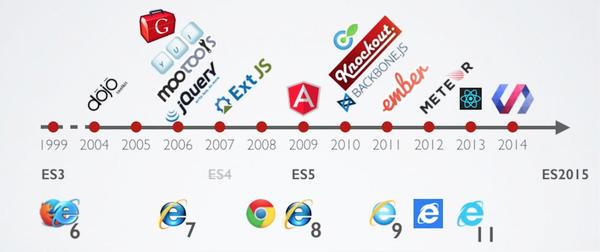
\includegraphics[scale=0.5]{images/history-of-frameworks.png}
	\end{center}
	\caption{Historical overview of JS frameworks and libraries}
\end{figure}

An application framework is defined as a large reusable collection of libraries, functions and tools in order application's main structure to be implemented. Thus, JavaScript frameworks are implementing the whole structure of an application, and make development of JS painless and faster by offering ready, optimized functions in comparison with native JS. Dependency management, file system structure and routing possibilities are also included. The term framework is used to declare that the execution flow of an application is handled by the framework and not the developer. This is the main difference between JS frameworks and libraries, since a library provides only a set of functionalities, while a framework conducts processing and data flow. (\cite{Reference6}) \par

Angular and ReactJS are nowadays widely scoped, full and continually improved JS frameworks or libraries, and their popularity have been significantly increased over time in front-end development. However, there is no framework or library considered to be as the best, a group of great choices exist that do have different functionalities and are selected based on some parameters that will be investigated in this thesis. (\cite{Reference6}) \par

\subsection{Data Architecture}

By developing dynamic pages, the need of application's data management was increased. For this reason, several data architectural patterns have been developed over time. At first, MVC pattern was used for a long period. MVC stands for Model-View-Controller, where model contains the business logic, view presents data through the user interface and controller connects the other two. However, MVC is not compiled into client side in the best way, fact that leads to the development of other data architectural approaches based on MVC for front-end. More specifically, there is MVW, or in other words \text{two-way data binding}, which means Model-View-Whatever. This pattern is used to describe Angular JS's architecture. MVW provide a common data structure in the application, and changes made in any area reflect the whole app. Another architectural approach is \textbf{Flux72}, which is an one-way data flow pattern. In this case, there are states that keep data and actions that change these data if needed, while views render what have been stored. Last but not least, there is the so called \text{Observable} pattern which is implemented from RxJs73 library. This is a publisher-subscriber architecture that provides streams of data. It includes functions for publishing values which are only executed in case subscribers exist. (\cite{murray2018ng}) \par

\subsubsection{Redux}

Redux is a library for data management in client side and was based on Facebook's Flux architectural approach, which was mentioned in previously as Flux72 pattern. (\cite{Reference13}) Managing data can be complicated when it comes to large apps. Intermediate passing of component state, the coupling between parent and child components that makes refactoring inflexible and the mismatching of state and DOM tree, are the reasons Redux was designed. (\citeyearpar{murray2018ng}) \par

More specifically, Redux is a Model-View-Controller library that handles data and interactions between layers inside an application. For this purpose, it is using reducers which are functions for computing application's state (\cite{Reference15}) and a global store that wraps all states of the application. In that way, data can be accessed and handled from any component, fact that unbinds UI from state changes, and reduces errors raised from state mismanagement. (\cite{Reference10}) \par

Redux is better described via three main principles. First of all, there is a single store, which mostly has the form of a JS object, and uses reducer functions for managing the small parts of the store. (\cite{Reference13}) In this way, it is easier to design and parse data through the application, and quick the process of debugging and testing. (\cite{Reference17}) The next principle is that state must not be modified by any component. For this purpose, reducer functions are used to build a new state when an action is provided without affecting the original state. Finally, the last principle is that reducers have to be functions that do not include API calls and do have deterministic results. (\cite{Reference13}) \par

\begin{figure}[h!]
	\begin{center}
		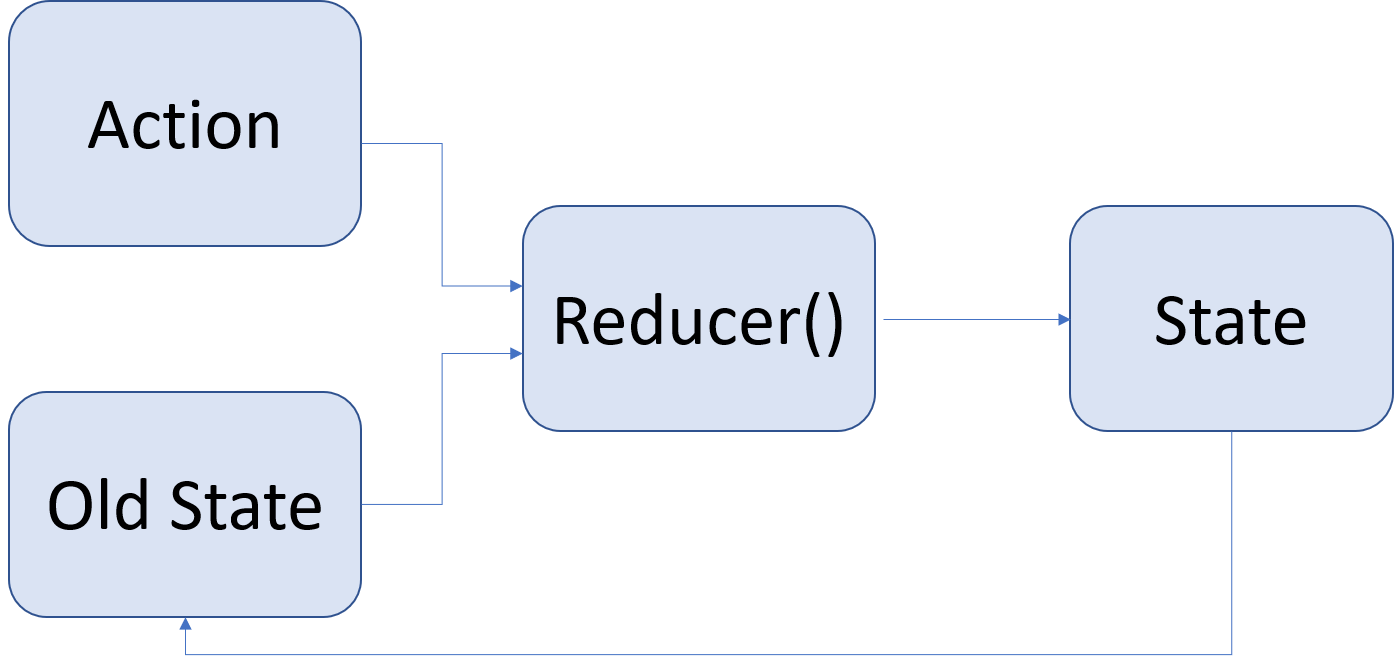
\includegraphics[scale=0.35]{images/Redux-Philosophy.png}
	\end{center}
	\caption{Redux Structure}
\end{figure}

To sum up, Redux is based on an architectural approach that provides scalability and tools for better data management. This library can be used in combination with other libraries or frameworks, like React and Angular, as it will mentioned in the next Chapters.

%\subsection{Webpack}
%Webpack, a tool which helps process and bundle our various JavaScript, CSS, HTML, and image files.(\cite{Reference10})

%Webpack is a module bundler that converts dynamic modules with dependencies into static assets. In application development, it is common to have various modules from either custom files or modules installed by Node Package Manager. These modules can contain one or multi- ple layers of dependencies. Webpack can bundle everything through a dependency graph, into a JavaScript file. Webpack also allow developers to export and import modules, code, and other assets between JavaScript files. Plugins and Loaders can be installed to extend Webpacks functionality. ??

%Many of the biggest frameworks consist of components. Components are the main building blocks of the framework. The way components are initialized and processed varies between the frameworks, but the main characteristics are the same: components can take information as parameters, perform actions, and possibly return some result. Components communicate with each other, can use each other’s properties and can have parents or child components. % frameworks +pros
%Components can be invisible to the user by doing only back-side processing. Or in turn, they can work with the user interface (UI) by producing an HTML document or part of it. Some frameworks utilize templates. Templates are initial HTML document files with an extended syntax of the framework itself. Components can take template as an input, make some changes and additions to it, and later output the completed HTML document. % components
%Components can exchange data with the server with Ajax requests. 

% 4 pages
